\documentclass[a4paper]{article}
\usepackage[colorlinks,linkcolor=black,urlcolor=black]{hyperref}
\usepackage{float}
\usepackage{mhchem}
\usepackage{pdfpages}
\usepackage{enumerate}
\usepackage{amsmath}
\usepackage{amssymb}
\usepackage{graphicx}
\usepackage{subfigure}
\usepackage{wrapfig}
\usepackage{geometry}
\usepackage{indentfirst}
\usepackage{array}
\usepackage{multirow} 
\usepackage{verbatim}
\setlength{\parindent}{2em}
\usepackage[greek,english]{babel} 
\geometry{left=2cm,right=2cm,top=1.5cm,bottom=1.5cm}

\begin{document}

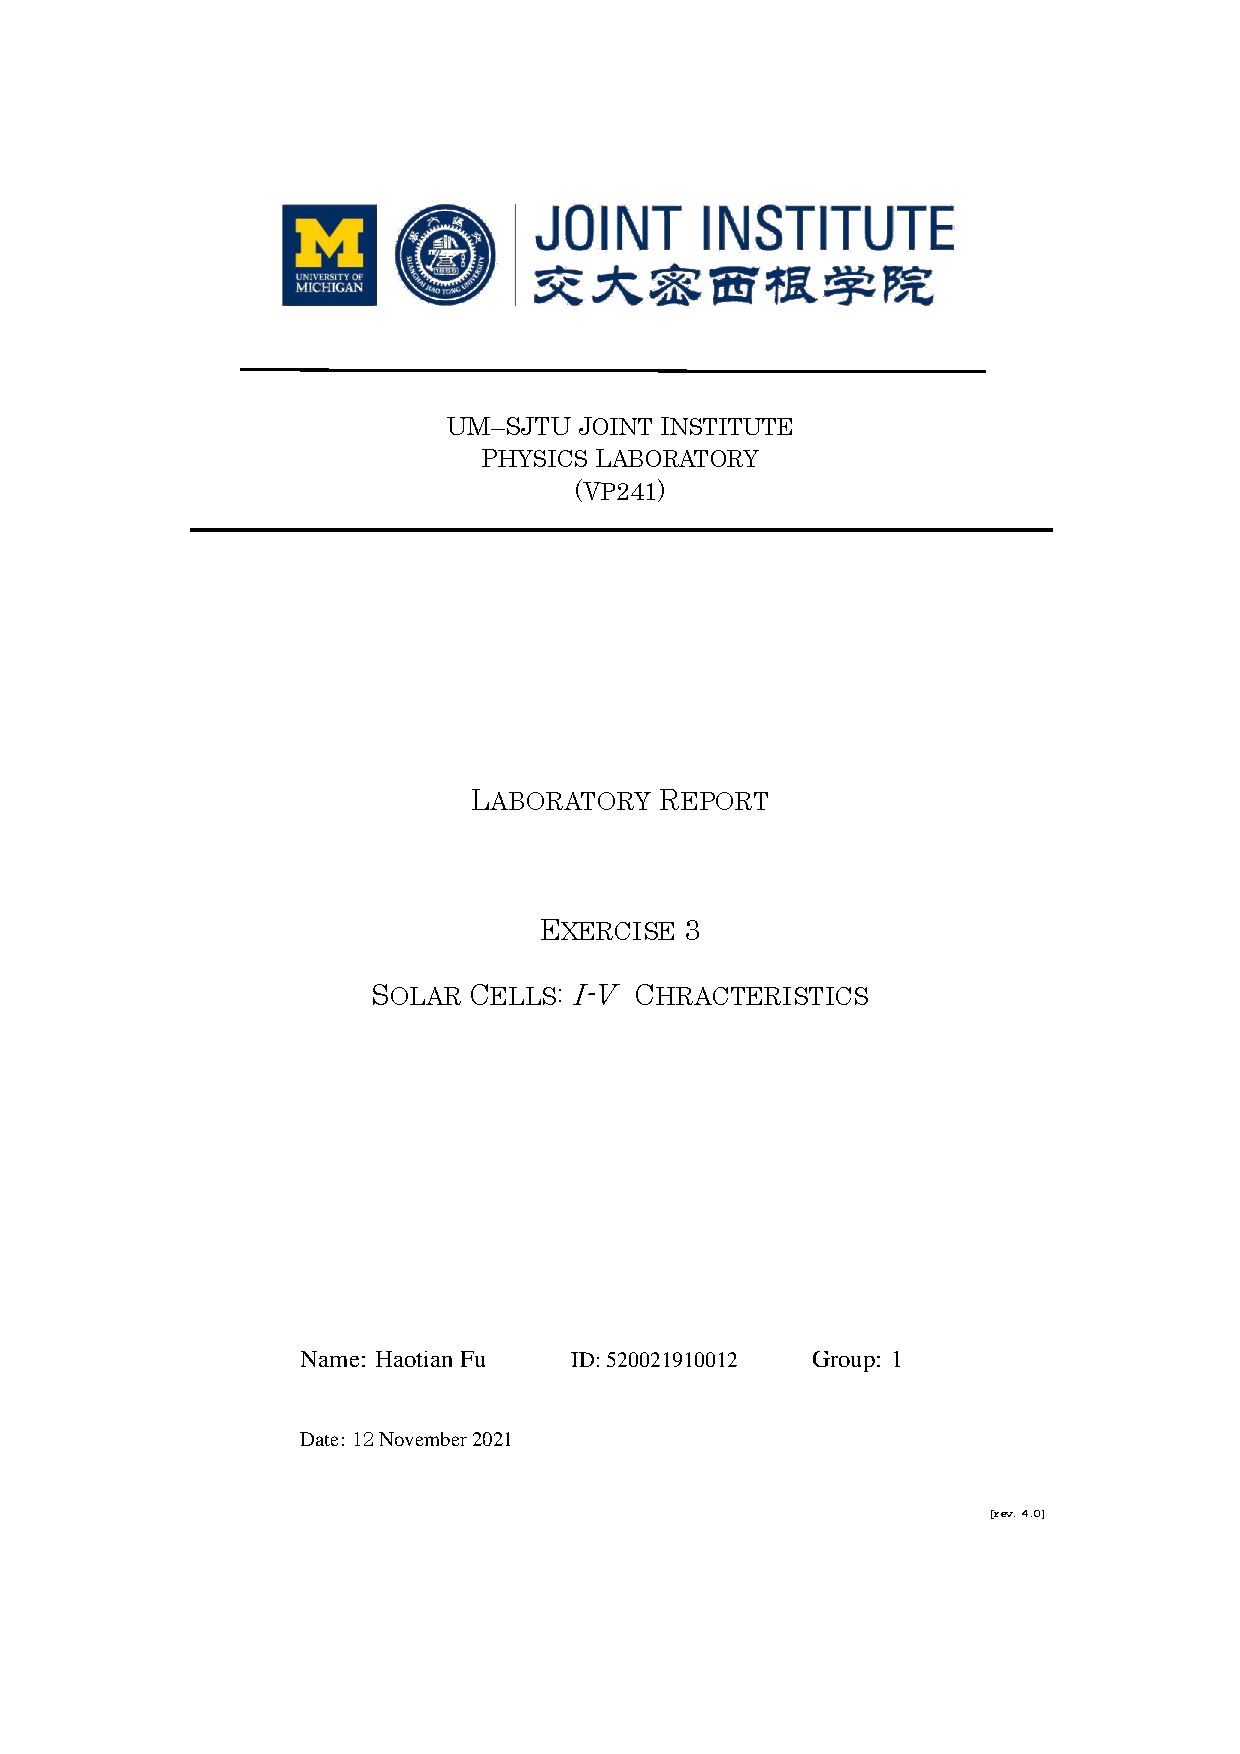
\includepdf{lab3_cover.pdf}

\newpage
\tableofcontents
\setcounter{page}{1}

\newpage
\listoffigures
\listoftables

\newpage
\section{Introduction}
The objective of this exercise is to urge students to be familiar with the working principle of a solar cell and study its current-voltage \textit{(I-V)} characteristics.

\subsection{Basic Concepts}
\begin{itemize}
	\item \textbf{Solar cell:}$^{[1]}$ Solar cells are devices which are able to directly transform solar radiation into electrical energy.
	      \begin{figure}[!htbp]
		      \centering
		      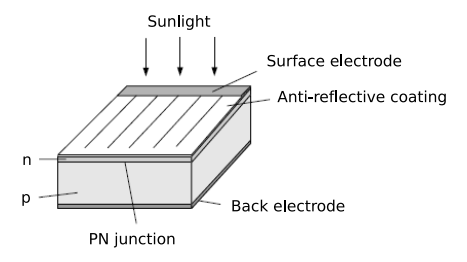
\includegraphics[width=0.45\textwidth]{solar_cell.png}
		      \caption{Solar cell}
	      \end{figure}
	\item \textbf{P-N junction:}$^{[2]}$ A p–n junction is a boundary or interface between two types of semiconductor materials, p-type and n-type, inside a single crystal of semiconductor.
	      \begin{figure}[!htbp]
		      \centering
		      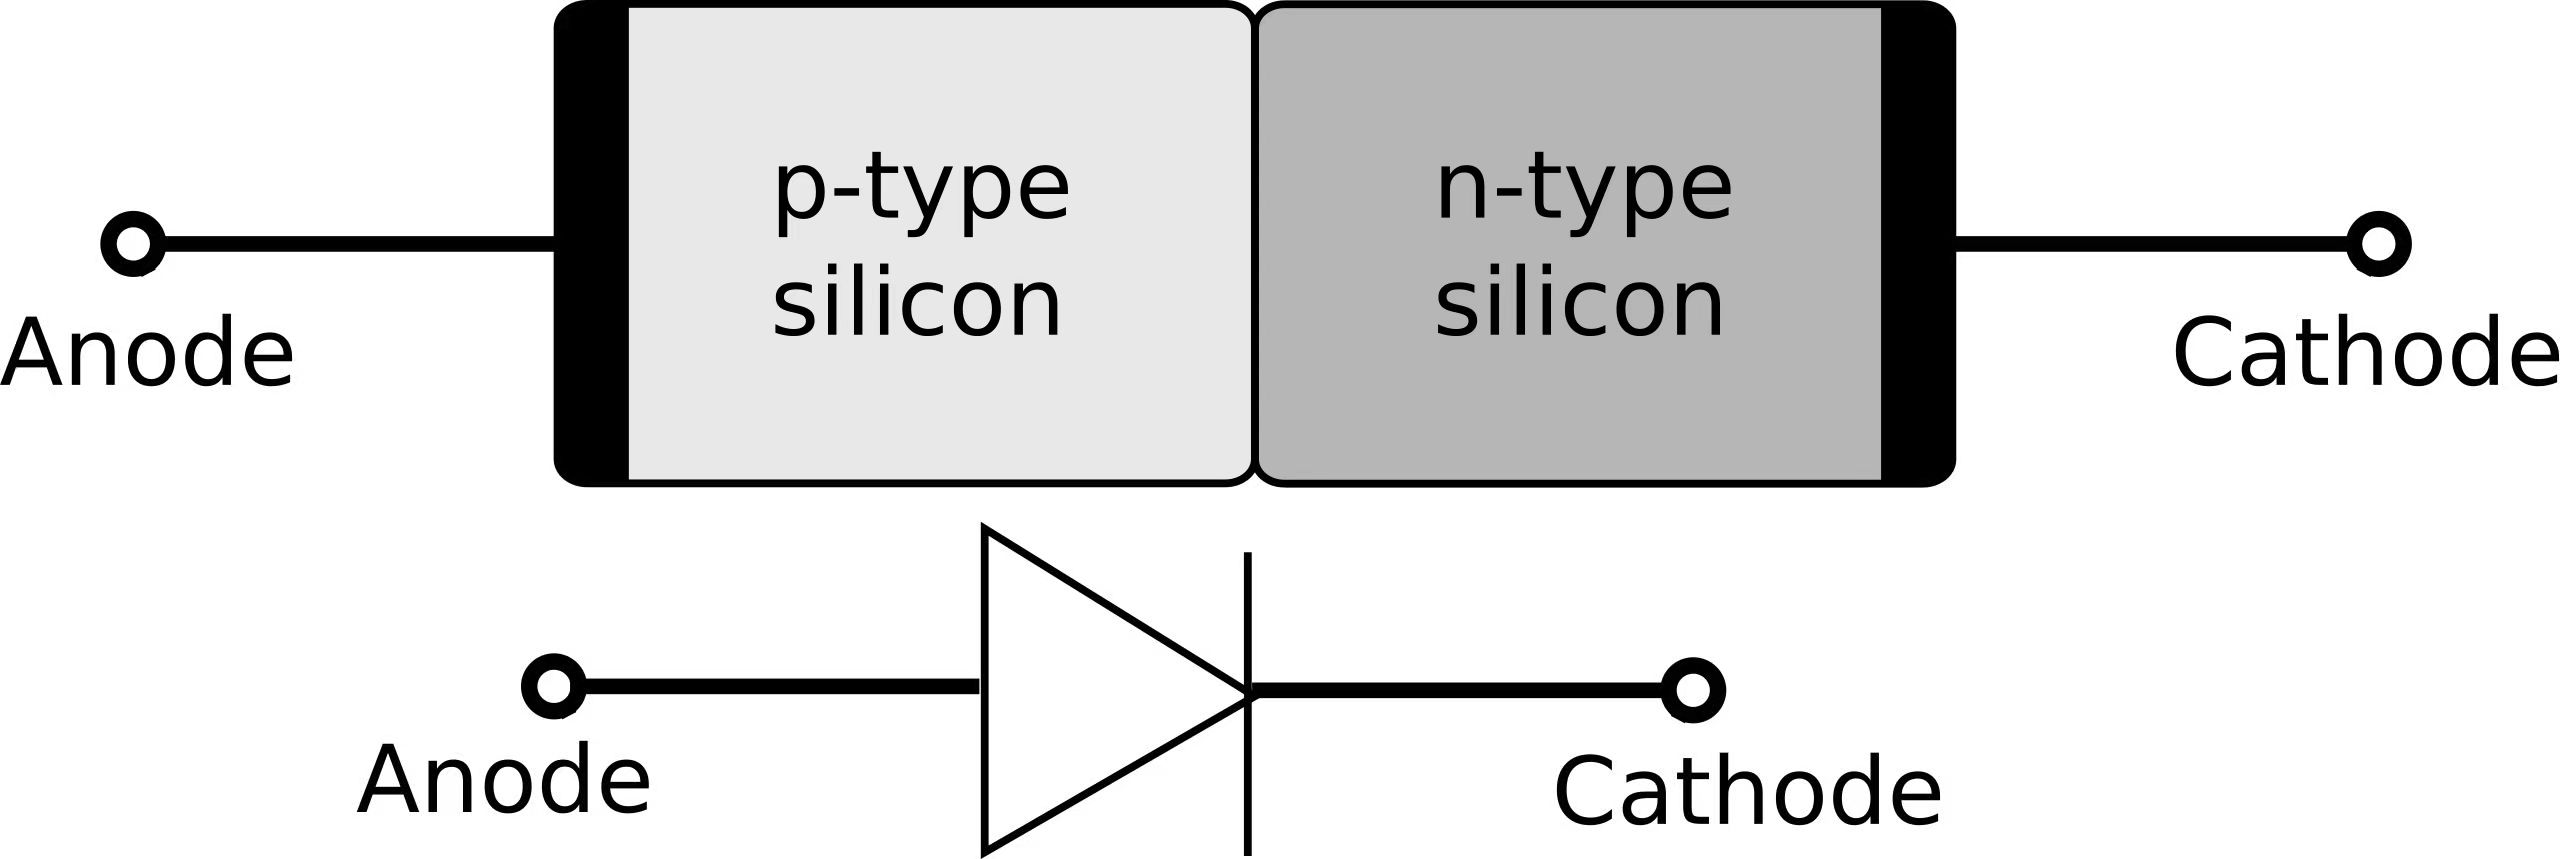
\includegraphics[width=0.4\textwidth]{pn_junction.jpg}
		      \caption{P-N junction}
	      \end{figure}
	\item \textbf{Photovoltaic (PV) effect:}$^{[3]}$ Photovoltaic (PV) effect is a process by which PV cell converts the absorbed sunlight energy into electricity.
	      \begin{figure}[!htbp]
		      \centering
		      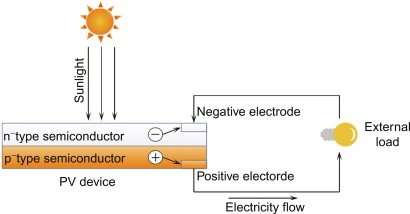
\includegraphics[width=0.5\textwidth]{photovoltaic_effect.jpg}
		      \caption{Photovoltaic effect}
	      \end{figure}
	\item \textbf{Fill factor:} Fill factor is the available power at the maximum power point ($P_\text{m}$) divided by the open circuit voltage ($V_\text{OC}$) and the short circuit current ($I_{\text{sc}}$).
	      \begin{equation}
		      F F=\frac{P_{\mathrm{m}}}{V_{\mathrm{oc}} I_{\mathrm{sc}}}=\frac{V_{\mathrm{m}} I_{\mathrm{m}}}{V_{\mathrm{oc}} I_{\mathrm{sc}}}
	      \end{equation}
	\item \textbf{Solar cell energy conversion efficiency:} The solar cell energy conversion efficiency $\eta$ is defined as
	      \begin{equation}
		      \eta=\frac{P_{\mathrm{m}}}{P_{\text {in }}} \times 100 \%
	      \end{equation}
	      where $P_{\text {in }}$ denotes the total radiant power incident on the solar cell while $P_\text{m}$ denotes the maximum output power.
\end{itemize}

\subsection{Theoretical Basis}
\subsubsection{The Principle of the Photovoltaic Effect$^{[1]}$}
\par When the light enters the $p-n$ junction near the solar cell surface, and the energy of
incident photons is greater than the forbidden bandwidth (energy gap) $E_g$, the incident
photons are absorbed and excite electron-hole pairs. Minority charge carriers in the $n-$ or
$p-$type area diffuse due to their density gradient. Some of them are able to diffuse to the
region of the $p-n$ junction where a built-in electric field exists. This field is directed from
the $n-$type to the $p-$type area. The minority carriers diffusing to the $p-n$ junction zone
between the $n-$type area and the $p-$type area are drawn by this electric field to the $p-$type
area (in case of the holes), or to the n-type area (in case of the electrons). This results in
an increase of positive charge accumulated in the p-type area and negative charge in the
$n-$type area. Consequently, a photoelectric potential difference is generated.


\subsubsection{Solar Cell Parameters}
\par The net current $I$ is
\begin{equation}
	I=I_{\mathrm{ph}}-I_{\mathrm{D}}=I_{\mathrm{ph}}-I_{0}\left[\exp \left(\frac{q V_{\mathrm{D}}}{n k_{\mathrm{B}} T}\right)-1\right]
	\label{eq::I}
\end{equation}
where $I_{\text{ph}}$ is the current from the $n-$type area to the $p-$area when there is light incident on the solar cell and $I_D$ is a forward diode current from the $p-$type to the $n-$type area, opposite to $I_{\text{ph}}$.
$V_D$ is the junction voltage, $I_0$ is the diode inverse saturation current, the coefficient $n$ is a theoretical coefficient, with its values ranging from 1 to 2, that characterizes the $p-n$ junction.
Furthermore, $q$ denotes the electron’s charge, $k_B$ is the Boltzmann’s constant, and $T$ is the temperature in the absolute (Kelvin) scale.

Ignoring the internal series resistance $R_s$, the voltage $V_D$ equals the terminal voltage $V$ and Eq.(\ref{eq::I}) can be rewritten as
\begin{equation}
	I=I_{\mathrm{ph}} - I_{0} \left[ \exp \left( \frac{q V}{n k_{\mathrm{B}} T}\right) - 1 \right]
	\label{eq::I_2}
\end{equation}

When the output is short, $i.e.$, $V=0$, the short-circuit current is
$$
	I_{\mathrm{sc}}=I_{\mathrm{ph}}
$$

whereas when the output is open, $i.e.$, $I=0$, the open-circuit voltage is
\begin{equation}
	V_{\mathrm{oc}}=\frac{n k_{\mathrm{B}} T}{q} \ln \left(\frac{I_{\mathrm{sc}}}{I_{0}}+1\right)
	\label{eq::V_OC}
\end{equation}

\subsubsection{Theoretical Graph}
\par Considering Eq.(\ref{eq::I_2}) and Eq.(\ref{eq::V_OC}), the corresponding $I-V$ characteristics curve is shown in Fig.(\ref{fig::theoretical_curve})
\begin{figure}[!htbp]
	\centering
	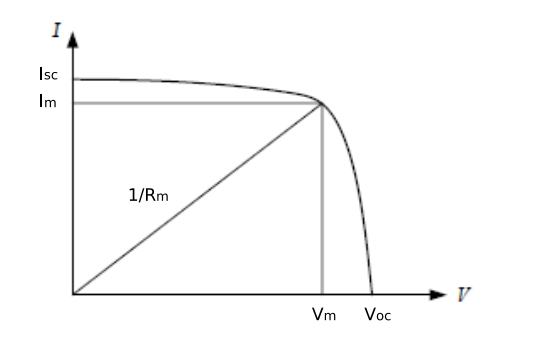
\includegraphics[width=0.6\textwidth]{theoretical_curve.png}
	\caption{The current-voltage characteristics of a solar cell.}
	\label{fig::theoretical_curve}
\end{figure}

\subsubsection{Solar Cell Equivalent Circuit}
\par As shown in Fig.(\ref{fig::equivalent_circuit}) , a solar cell can be thought of as composed of a $p-n$ junction diode $D$ and a constant current source $I_{\mathrm{ph}}$. Along with a series resistance $R_{\mathrm{s}}$ due to the electrodes in the solar cell and a parallel resistance $R_{\mathrm{sh}}$, all elements form a circuit equivalent to a $p$ - $n$ junction leak-circuit. For the equivalent circuit one can find the following relationship between the current and the voltage
$$
	I=I_{\mathrm{ph}}-I_{0}\left\{\exp \left[\frac{q\left(V+R_{\mathrm{s}} I\right)}{n k_{\mathrm{B}} T}\right]-1\right\}-\frac{V+R_{\mathrm{s}} I}{R_{\mathrm{sh}}}
$$
\begin{figure}[!htbp]
	\centering
	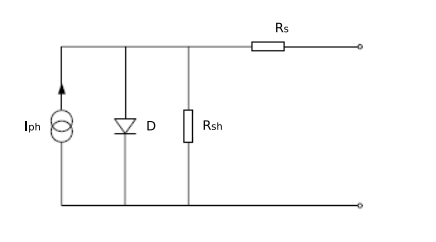
\includegraphics[width=0.5\textwidth]{equivalent_circuit.png}
	\caption{Solar cell equivalent circuit.}
	\label{fig::equivalent_circuit}
\end{figure}

\section{Apparatus and Measurement Procedure}

\subsection{Apparatus}
The setup consists of a photovoltaic device (5 W), a 300 W tungsten-halogen lamp
serving as a radiation source, two digital multimeters, two adjustable resistors, a solar
power meter, a wiring board and a measuring tape.

The precisions of the devices are shown in Table \ref{table::Precision}.
\begin{table}[htbp]
	\centering
	\begin{tabular}{cc}
		\hline
		Instrument  & Uncertainties          \\
		\hline
		DC Voltage  & $\pm (0.5\%+0.01)\,$V  \\
		DC Current  & $\pm (1.5\% + 0.1\,$mA \\
		Distance    & $\pm 0.1\%\,$cm        \\
		Solar power & $\pm 10\,$W/cm$^2$     \\
		\hline
	\end{tabular}
	\caption{Information of measurement instruments.}
	\label{table::Precision}
\end{table}

\subsection{Measurement Procedure}

In this exercise, the characteristics of four configurations of the solar cell are studied. For each configuration, the $I-V$ $P-V$, $P-R$ relations are studied and for each single configurations, the information about fill factor and energy conversion efficiency are also explored.
\begin{enumerate}
    \item Turn on both the light and the fan and then wait until the light reaches its working intensity.
    \item Design a measuring circuit with the photovoltaic device, multimeters set in an appropriate range, and the resistance. Connect the elements into a circuit using the provided wiring board.
    \item Adjust the distance between the light source and the photovoltaic device until the $V_\text{oc}$ and $I_\text{sc}$ of the two devices are about the same. Measure the solar power by the provided solar power meter.
    \item Change the distance between the light source and the photovoltaic device and measure the $I-V$ characteristics curves and the values of $V_\text{oc}$ and $I_\text{sc}$ in a single-device configuration. Measure the solar power at this distance.
    \item Plot
\end{enumerate}

\subsection{Safety Notice}

\begin{itemize}
	\item The temperature of the light source is very high, do not touch the cover.
	\item The power supply voltage of the light source is 220 V, beware of electric shock.
\end{itemize}


\section{Experimental Results}



\section{Uncertainty Analysis}

\subsection{Relationship Between Sensitivity $K_H$ and Working Voltage $U_S$}
According to Table \ref{table::initial}, the uncertainties are calculated as
\begin{align*}
	u_{U_\text{S}}  & = 5.00\times 0.5\% = 0.03\ [\text{V}]                          \\
	u_{U_0}         & = 2.504\times0.05\%+6\times10^{-3} = 0.007\ [\text{V}]         \\
	u_U             & = 2.621\times0.05\%+6\times10^{-3} = 0.007\ [\text{V}]         \\
	u_{I_\text{M2}} & = 250 \times 10^{-3} \times 2\% = 5 \times 10^{-3}\ [\text{A}]
\end{align*}
while $B(x=0,I_\text{M}=250\ [\text{mA}]) = \frac{I_\text{M2}}{I_{\text{M1}}} \times B(x=0,I_\text{M}=100\ [\text{mA}])$
\begin{equation*}
	u_B = \frac{B(x=0,I_\text{M}=100\ [\text{mA}])}{I_{\text{M1}}}u_{I_\text{M2}} = \frac{1.4366\times 10^{-3}}{100\times 10^{-3}} \times 5\times 10^{-3} = 7 \times 10^{-5}\ [\text{T}]
\end{equation*}
\par Then for $K_\text{H} = \frac{U-U_0}{B}$, its uncertainty is
\begin{align*}
	u_{K_\text{H}} & = \sqrt{(\frac{\partial K_\text{H}}{\partial U}u_U)^2+(\frac{\partial K_\text{H}}{\partial U_0}u_{U_0})^2+(\frac{\partial K_\text{H}}{\partial B}u_B)^2} = \sqrt{(\frac{u_U}{B})^2+(\frac{-u_{U_0}}{B})^2+(-\frac{(U-U_0)u_B}{B^2})^2} \\
	               & =\sqrt{(\frac{0.007}{1.4366\times10^{-3}\times250/100})^2+(\frac{-0.007}{1.4366\times10^{-3}\times250/100})^2+(\frac{(2.621-2.504)\times 7\times 10^{-5}}{(1.4366\times10^{-3}\times250/100)^2})^2}                                    \\
	               & =3\ [\text{V}/\text{T}].
\end{align*}

For Table \ref{table::e1}, the uncertainties of data for voltage measurements are calculated as follows. Take the first set of data as an example,
$$u_{U_\text{S}} = 2.80\times 0.5\% = 0.014\,\,[\text{V}],$$
$$u_{U_0} = 1.4004\times0.05\%+6\times10^{-4} = 0.0013\,\,[\text{V}],$$
$$u_U = 1.4656\times0.05\%+6\times10^{-4} = 0.0014\,\,[\text{V}].$$

The uncertainty for $ K_\text{H}/U_\text{S} = \frac{U-U_0}{BU_\text{S}} $ is calculated as
\begin{align*}
	u_{K_\text{H}/U_\text{S}} & = \sqrt{(\frac{\partial K_\text{H}/U_\text{S}}{\partial U}u_U)^2+(\frac{\partial K_\text{H}/U_\text{S}}{\partial U_0}u_{U_0})^2+(\frac{\partial K_\text{H}/U_\text{S}}{\partial U_\text{S}}u_{U_\text{S}})^2+(\frac{\partial K_\text{H}/U_\text{S}}{\partial B}u_B)^2} \\
	                          & = \sqrt{(\frac{u_U}{BU_\text{S}})^2+(\frac{-u_{U_0}}{BU_\text{S}})^2+(-\frac{U-U_0}{BU_\text{S}^2}u_{U_\text{S}})^2+(-\frac{U-U_0}{B^2U_\text{S}}u_{B})^2}                                                                                                             \\
	                          & = \sqrt{(\frac{0.0014}{3.59\times10^{-3}\times2.80})^2+(\frac{-0.0013}{3.59\times10^{-3} \times2.80})^2+(-\frac{(1.4656-1.4004)\times 0.014}{3.59\times10^{-3} \times 2.80^2})^2+(-\frac{(1.4656-1.4004)\times 7\times 10^{-5}}{{(3.59\times 10^{-3})}^2 \times 2.80}} \\
	                          & =0.2\ [\text{T}^{-1}].
\end{align*}

The uncertainties of all other data in Table \ref{table::e1} are calculated in this way and the results are presented in Table \ref{table::ue1}.

\begin{table}[H]
	\centering
	\begin{tabular}{crrrc}
		\hline
		   & $u_{U_\text{S}}\,\,[\text{V}]$ & $u_{U_0}\,\,[\text{V}]$ & $u_U\,\,[\text{V}]$ & $u_{K_\text{H}/U_\text{S}}\,\,[\text{T}^{-1}]$ \\
		\hline
		1  & 0.014                          & 0.0013                  & 0.0014              & 0.2                                            \\
		2  & 0.016                          & 0.0014                  & 0.0015              & 0.2                                            \\
		3  & 0.018                          & 0.0015                  & 0.0016              & 0.2                                            \\
		4  & 0.020                          & 0.007                   & 0.007               & 0.2                                            \\
		5  & 0.022                          & 0.008                   & 0.008               & 0.5                                            \\
		6  & 0.024                          & 0.008                   & 0.008               & 0.6                                            \\
		7  & 0.026                          & 0.008                   & 0.008               & 0.6                                            \\
		8  & 0.028                          & 0.008                   & 0.008               & 0.5                                            \\
		9  & 0.030                          & 0.008                   & 0.008               & 0.5                                            \\
		10 & 0.032                          & 0.008                   & 0.008               & 0.5                                            \\
		11 & 0.034                          & 0.008                   & 0.008               & 0.5                                            \\
		12 & 0.036                          & 0.008                   & 0.008               & 0.4                                            \\
		13 & 0.038                          & 0.008                   & 0.008               & 0.4                                            \\
		14 & 0.040                          & 0.008                   & 0.008               & 0.4                                            \\
		15 & 0.042                          & 0.008                   & 0.009               & 0.4                                            \\
		16 & 0.044                          & 0.009                   & 0.009               & 0.3                                            \\
		17 & 0.046                          & 0.009                   & 0.009               & 0.3                                            \\
		18 & 0.050                          & 0.009                   & 0.009               & 0.3                                            \\
		\hline
	\end{tabular}
	\caption{Uncertainties of data in Table \ref{table::e1}.}
	\label{table::ue1}
\end{table}

\subsection{Uncertainty of Input Current $I_\text{M}$, Output Voltage $U$ and Magnetic Field $B$}

Take the last set of data in Table \ref{table::IMU} as an example.\\

The uncertainty for $I_\text{M}$ is
$$u_{I_\text{M}} = 0.50\times 2\% = 0.010\,\,[\text{A}]$$

The uncertainty for $U$ is
$$u_U = 231.1\times 0.05\%+6\times10^{-3} = 0.12\,\,[\text{mV}].$$

The uncertainties of all other data in Table \ref{table::IMU} are calculated in this way are the results are presented in Table \ref{table::uIMU}.

\begin{table}[H]
	\centering
	\begin{tabular}{ccc}
		\hline
		   & $u_{I_\text{M}}\,\,[\text{A}]$ & $u_{U_{\text{out}}}\,\,[\text{V}]$ \\
		\hline
		1  & 0                              & 0.007                              \\
		2  & 0.001                          & 0.03                               \\
		3  & 0.002                          & 0.04                               \\
		4  & 0.003                          & 0.05                               \\
		5  & 0.004                          & 0.06                               \\
		6  & 0.005                          & 0.07                               \\
		7  & 0.006                          & 0.08                               \\
		8  & 0.007                          & 0.09                               \\
		9  & 0.008                          & 0.10                               \\
		10 & 0.009                          & 0.12                               \\
		11 & 0.010                          & 0.13                               \\
		\hline
	\end{tabular}
	\caption{Uncertainty of data in Table \ref{table::IMU}.}
	\label{table::uIMU}
\end{table}

\subsection{Uncertainty of Magnetic Field Inside the Solenoid Measurement}

The uncertainty of position measurement is 0.05 cm.

As for the uncertainty of the output voltage, taking the first set of data as an example,
$$u_U = 12.20 \times 0.05\% + 6\times 10^{-3} = 0.012\ \text{[mV]}$$

Due to $B(x) =\frac{U}{K_\text{H}}$,
$$ u_B = \sqrt{(\frac{\partial B}{\partial U}u_U)^2 + (\frac{\partial B}{\partial K_\text{H}}u_{K_\text{H}})^2} = \sqrt{(\frac{u_U}{K_\text{H}})^2 + (-\frac{U}{K_\text{H}^2}u_{K_\text{H}})^2}. $$

Taking the first set of data as an example,
$$  u_B = \sqrt{(\frac{0.012\times 10^{-3}}{33.6})^2 + (-\frac{12.20\times 10^{-3}}{33.6^2}\times 0.7)^2} = 0.008 \times10^{-3}\,[\text{T}]. $$

The uncertainties for all other sets of data are calculated and shown in Table \ref{table::uUB}.

\begin{table}[htbp]
	\centering
	\begin{tabular}{ccc||ccc}
		\hline
		   & $u_U\,\,[\text{mV}]$ & $B(x)\,\,[10^{-3}\,\,\text{T}]$ &    & $u_U\,\,[\text{mV}]$ & $B(x)\,\,[10^{-3}\,\,\text{T}]$ \\
		\hline
		1  & 0.012                & 0.008                           & 27 & 0.07                 & 0.08                            \\
		2  & 0.014                & 0.010                           & 28 & 0.07                 & 0.08                            \\
		3  & 0.016                & 0.013                           & 29 & 0.07                 & 0.08                            \\
		4  & 0.02                 & 0.017                           & 30 & 0.07                 & 0.08                            \\
		5  & 0.03                 & 0.03                            & 31 & 0.07                 & 0.08                            \\
		6  & 0.04                 & 0.04                            & 32 & 0.07                 & 0.08                            \\
		7  & 0.05                 & 0.05                            & 33 & 0.07                 & 0.08                            \\
		8  & 0.05                 & 0.06                            & 34 & 0.07                 & 0.07                            \\
		9  & 0.06                 & 0.06                            & 35 & 0.07                 & 0.07                            \\
		10 & 0.06                 & 0.07                            & 36 & 0.07                 & 0.07                            \\
		11 & 0.06                 & 0.07                            & 37 & 0.06                 & 0.07                            \\
		12 & 0.07                 & 0.07                            & 38 & 0.06                 & 0.07                            \\
		13 & 0.07                 & 0.07                            & 39 & 0.06                 & 0.06                            \\
		14 & 0.07                 & 0.07                            & 40 & 0.06                 & 0.06                            \\
		15 & 0.07                 & 0.07                            & 41 & 0.05                 & 0.06                            \\
		16 & 0.07                 & 0.07                            & 42 & 0.05                 & 0.05                            \\
		17 & 0.07                 & 0.07                            & 43 & 0.05                 & 0.05                            \\
		18 & 0.07                 & 0.07                            & 44 & 0.05                 & 0.05                            \\
		19 & 0.07                 & 0.07                            & 45 & 0.04                 & 0.04                            \\
		20 & 0.07                 & 0.08                            & 46 & 0.04                 & 0.04                            \\
		21 & 0.07                 & 0.08                            & 47 & 0.04                 & 0.03                            \\
		22 & 0.07                 & 0.08                            & 48 & 0.03                 & 0.03                            \\
		23 & 0.07                 & 0.08                            & 49 & 0.03                 & 0.03                            \\
		24 & 0.07                 & 0.08                            & 50 & 0.03                 & 0.02                            \\
		25 & 0.07                 & 0.08                            & 51 & 0.03                 & 0.018                           \\
		26 & 0.07                 & 0.08                            & 52 & 0.019                & 0.016                           \\
		\hline
	\end{tabular}
	\caption{The uncertainties of $U$ and $B$.}
	\label{table::uUB}
\end{table}

\section{Conclusion and Discussion}

\subsection{Conclusion}

In this exercise, we learnt how to use integrated Hall probe and measured the Hall sensitivity of the Hall probe under different working voltages.
Besides, we derived two experimental value of $K_H$ in two different ways, where one is direct measurement and the other is linear fit.
We also measured the magnetic field inside a solenoid. Among all the steps and operations, we conclude that
\begin{itemize}
	\item As Fig.(\ref{fig::KHUS}) suggests, the sensitivity has a decreasing trend with working voltage increasing.
	\item The output voltage is probably linearly dependent on the magnetic field since the Pearson's r of linear fit
	      in Fig.(\ref{fig::linear fit}) is 0.998 which is very close to 1.
	\item The $K_H$ we measure is quite precise since the relative error is only $\frac{33.6-31.25}{31.25}\times 100\% = 7.52\%$.
	\item The magnitudes of measured magnetic field and theoretical magnetic field differ a bit but with a raltively constant difference throughout
	      the whole curve.
\end{itemize}
\par The detailed analysis will be presented in Discussion part.

\subsection{Discussion}

\subsubsection{Problems}
\begin{enumerate}[1.]
	\item As for the relationship between sensitivity of SS495A and the working voltage applied on it, it is
	      positively proportional in fact$^{[4]}$, which contradicts the data we derived in this exercise.
	\item Measured data has relatively great deviation of theoretical value as Fig.(\ref{fig::theo_and_meas})
	      suggests.
\end{enumerate}

\subsubsection{Potential errors}
\par Here we conclude some potential errors occuring in this exercise.
\begin{enumerate}[1.]
	\item Uneven Hall Probe \\
	      \par The materials consisting of the integrated Hall probe may not be so even that there will also trigger
	      electric field even if there is no magnetic field applied. This magnetic filed triggered by the material itself
	      may be opposite to the magnetic filed applied, which will leesen the magnitude of magnetic field we detected.
	\item Ettingshausen effect and Nernst effect \\
	      \par Due to Hall effect, electrons are forced to move perpendicular to the applied current. However,
	      the accumulation of electrons on one side of the sample enables the number of collisions to increase and a
	      heating of the material occurs, which will trigger a heated electromotive force. This emf will decrease the the
	      effect of origin current in converse.
	\item Reading Process \\
	      \par The sensibility of the experiment device is so low that we can hardly grasp a more precise number about two digits
	      after the decimal point. The reading process may cause huge deviation due to the unstability of the data displayed.
\end{enumerate}

According to the above discussion, we may explain the difference between data we measured and the theoretical value.
In general, the results we derived are still credible and worthy. Here we also provide some suggestions to impove.

\subsubsection{Imporvements}
\begin{itemize}
	\item Use more precise experiment devices.
	\item Control the experimental temperature better to avoid temperarture deviation.
	\item Cool down the integrated Hall probe as we measure the data.
\end{itemize}



\newpage
\section{Reference}
\noindent [1] M. Krzyzosiak (2021). Exercise 3 - lab manual [rev 5]. (UMJI-SJTU, Shanghai). \\
\noindent [2] \url{https://en.wikipedia.org/wiki/P–n_junction} \\
\noindent [3] \url{https://www.sciencedirect.com/topics/engineering/photovoltaic-effect} \\
\noindent [4] Sinocomopto Technologies Ltd. Company, \textit{SS495A Product Manual}, Archived from the original on 2021-11-11.


\newpage
\section*{APPENDIX - DATA SHEET}

%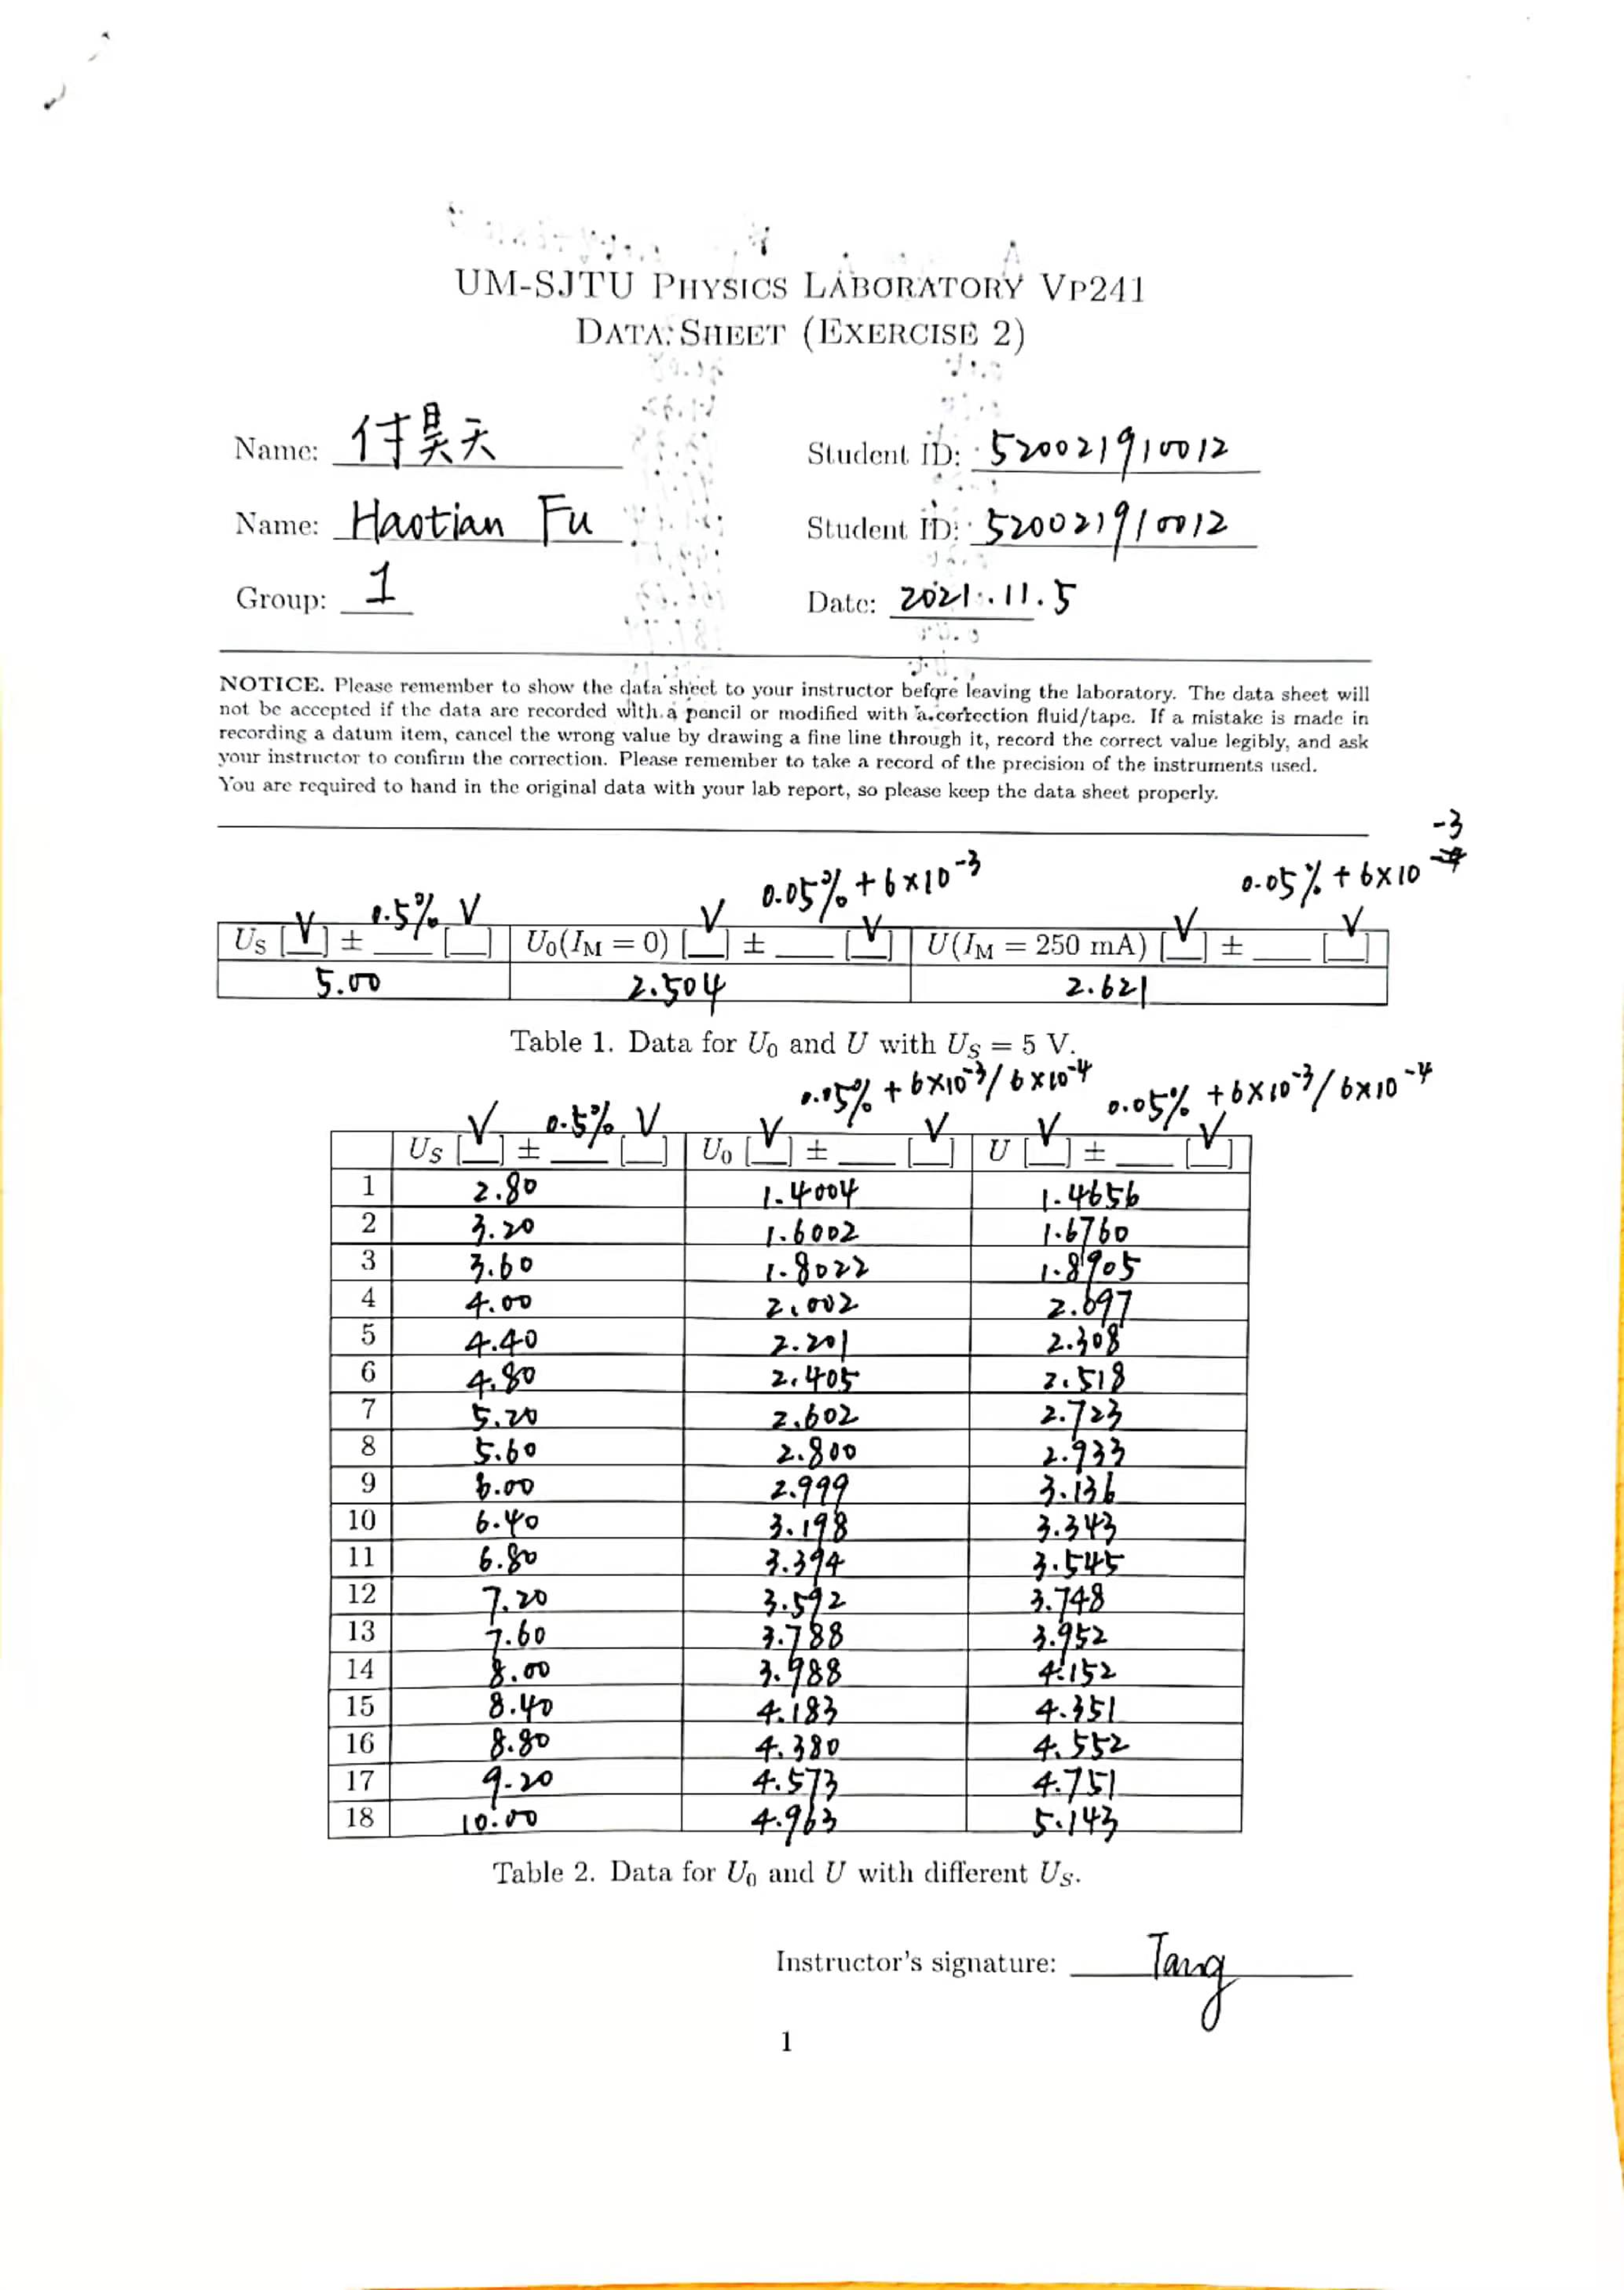
\includepdf{data_sheet_1.pdf}
%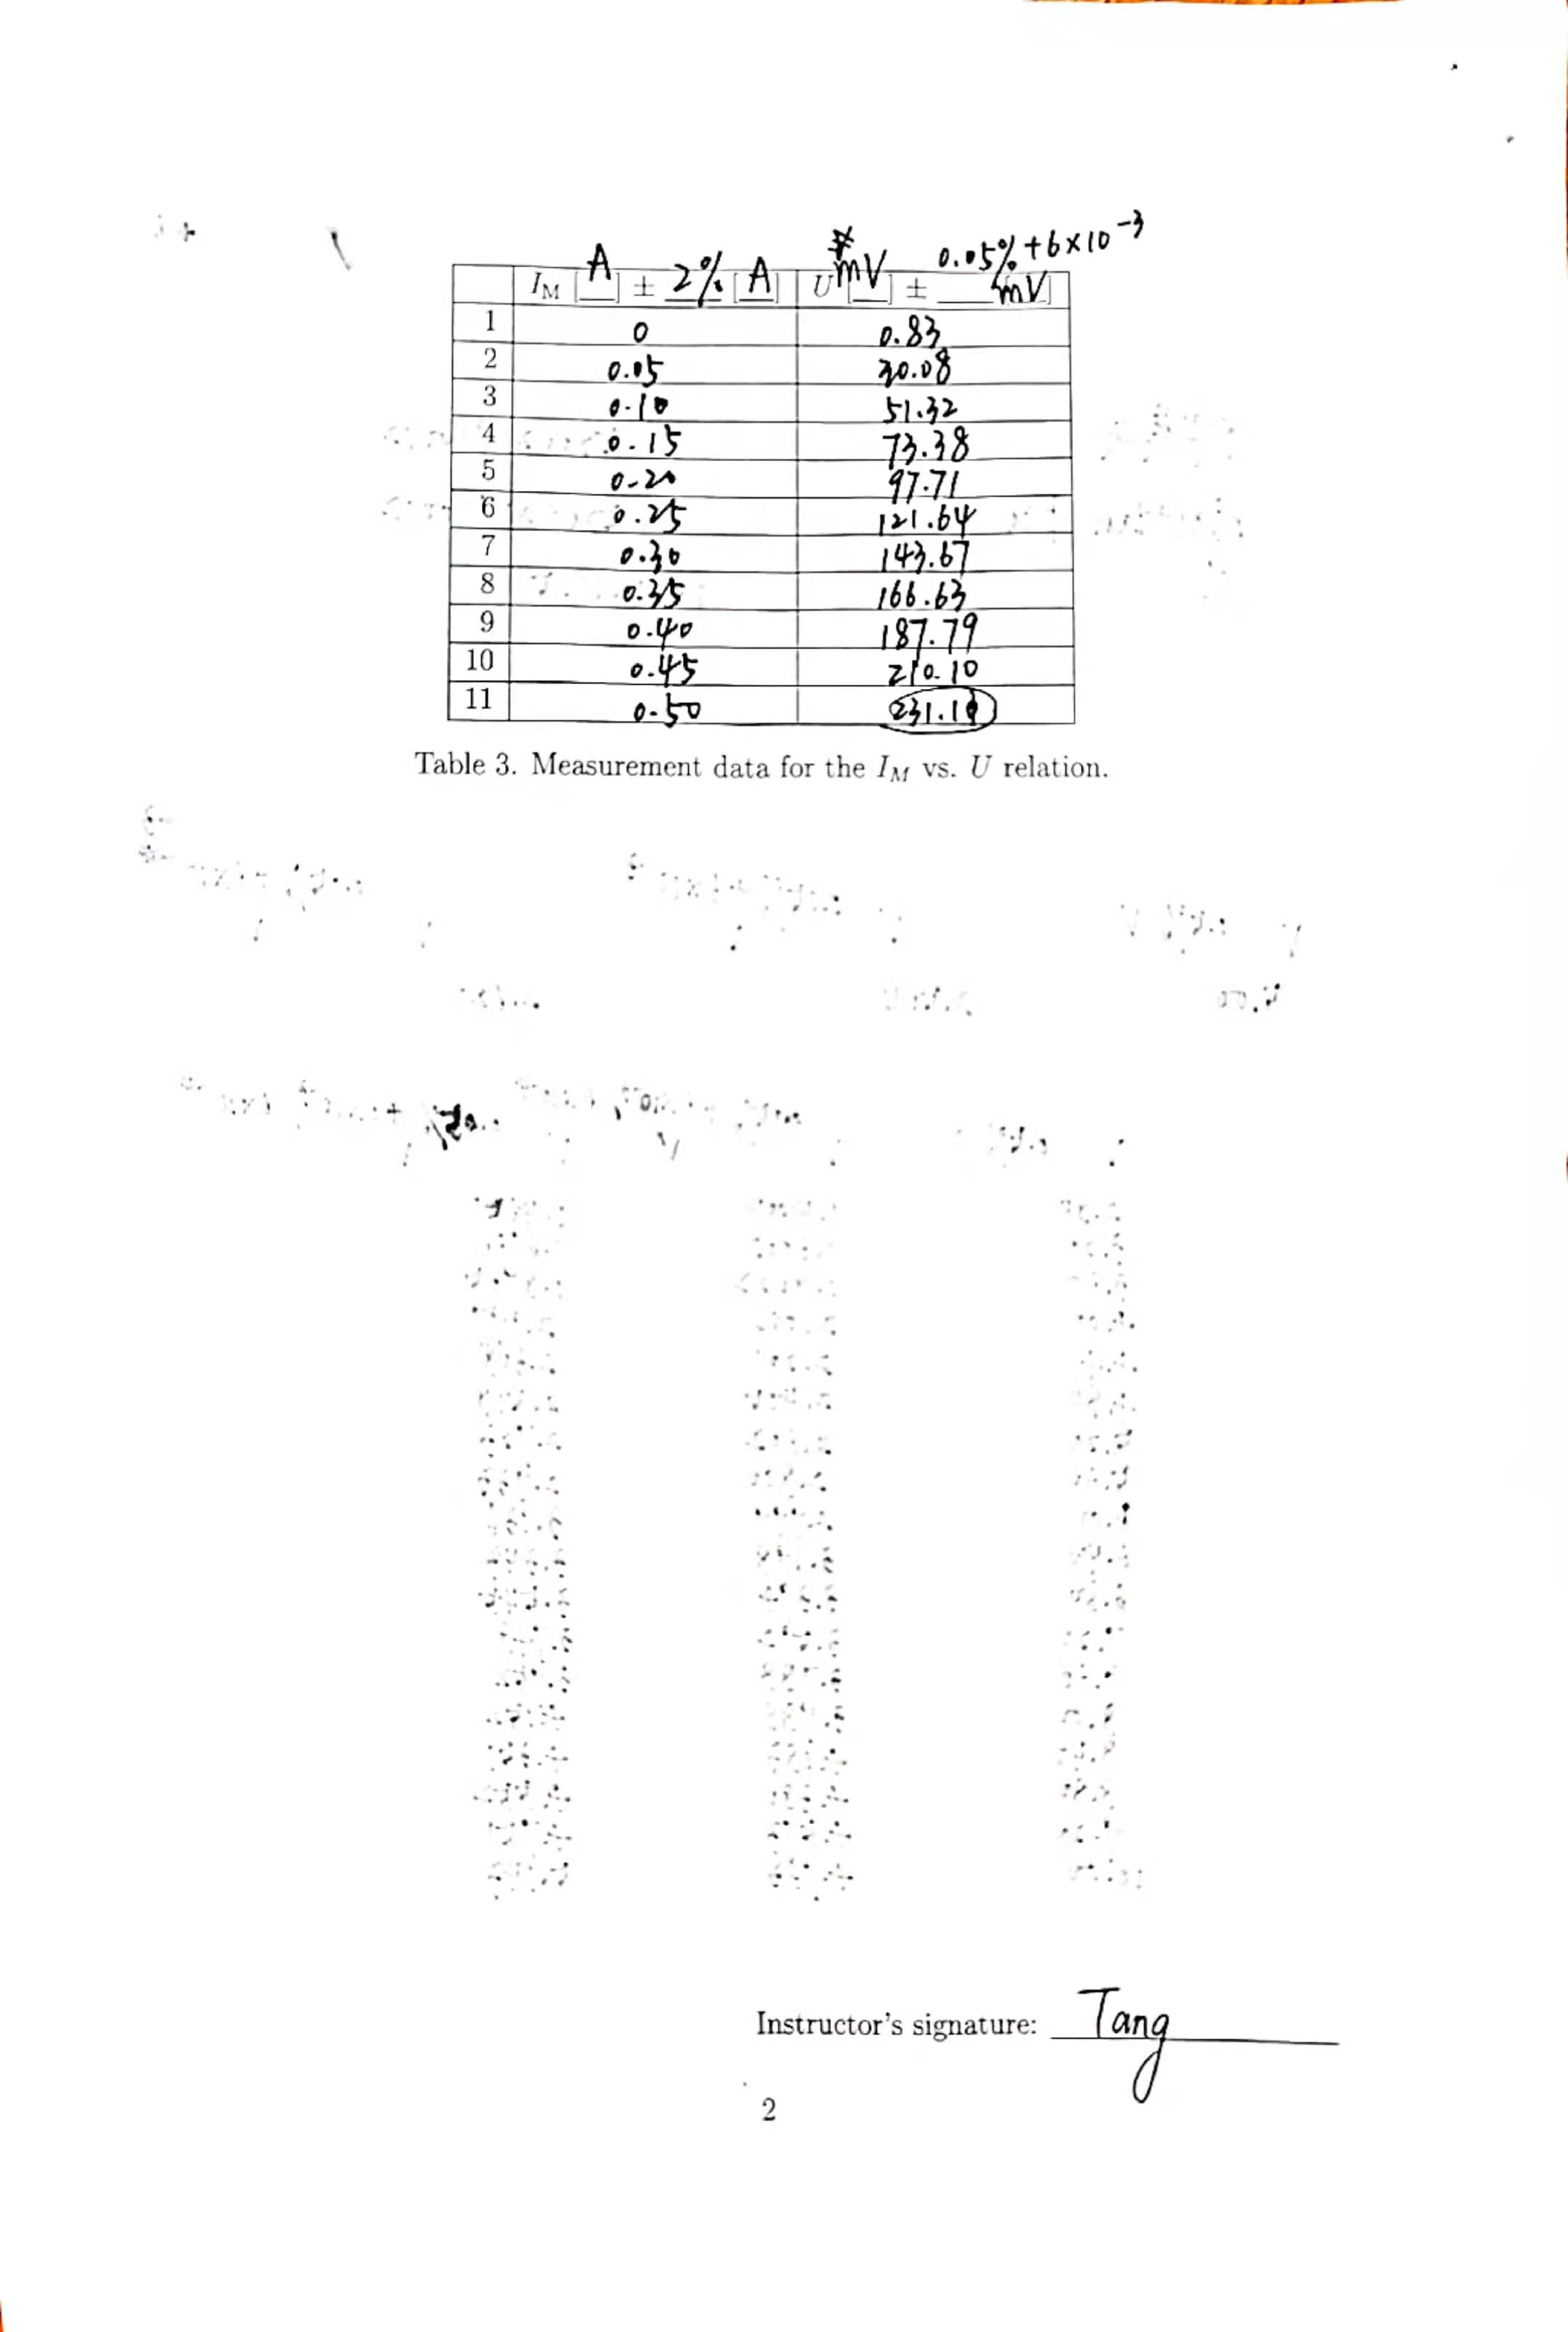
\includepdf{data_sheet_2.pdf}
%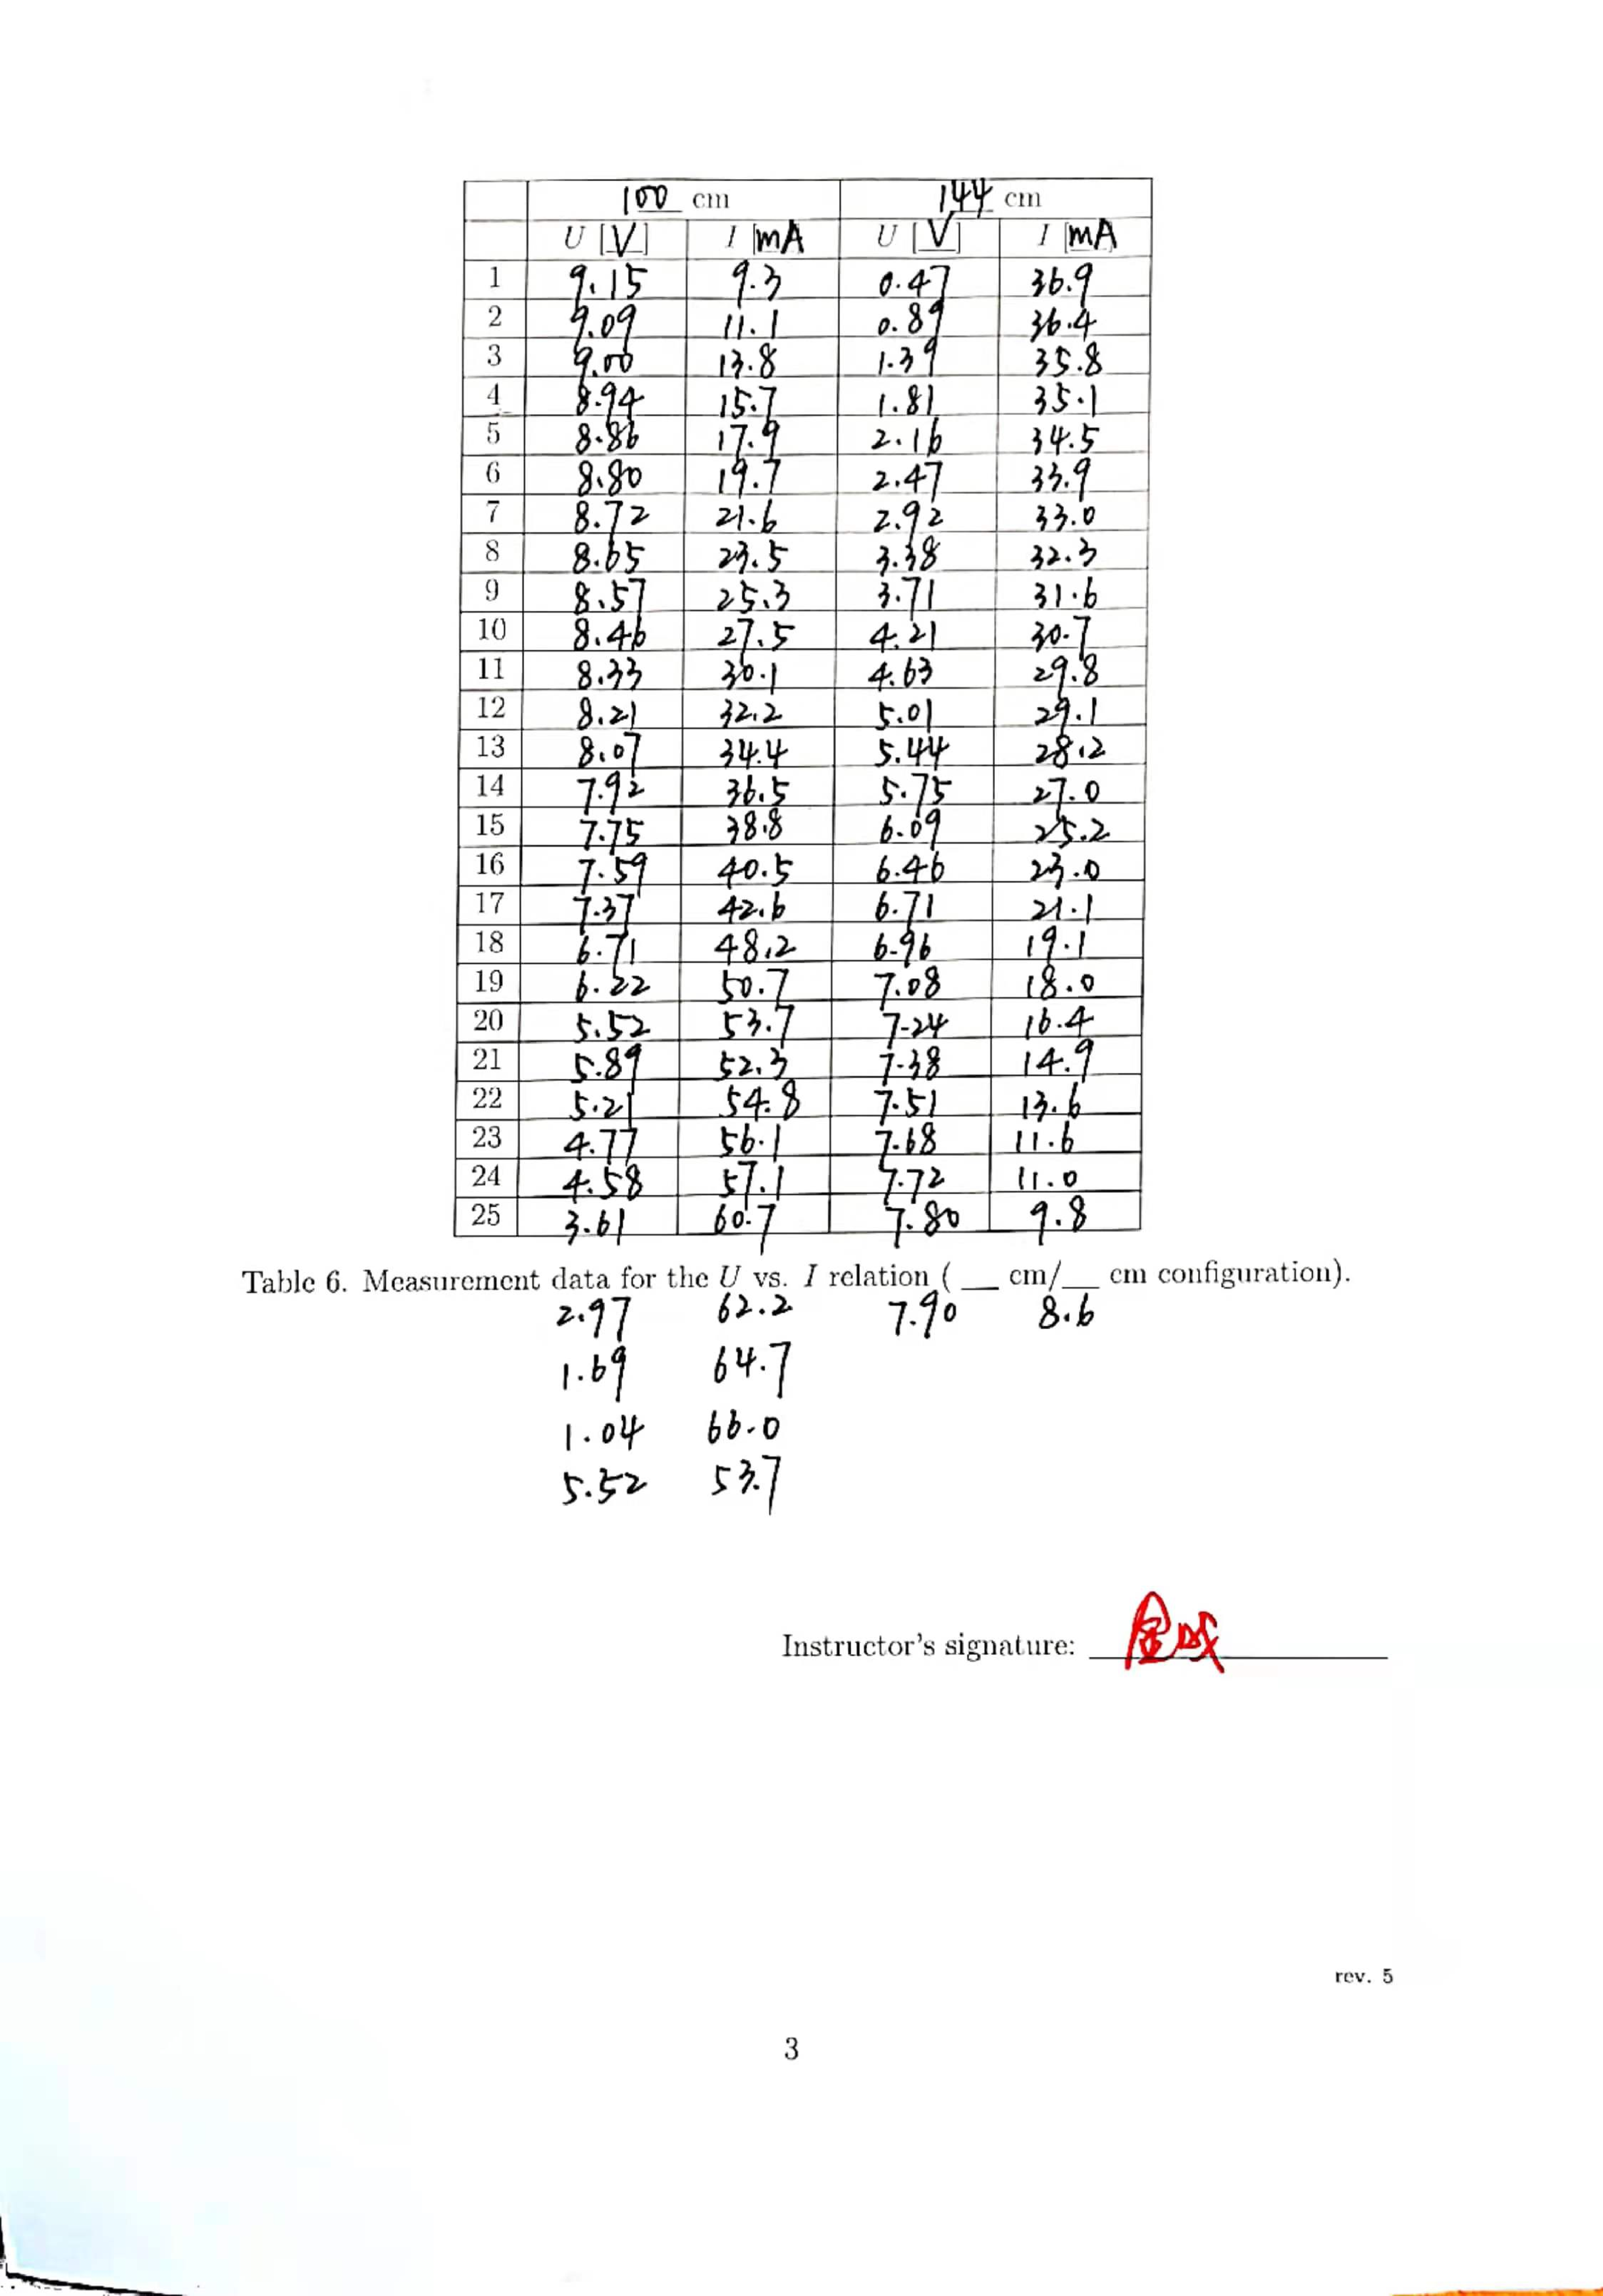
\includepdf{data_sheet_3.pdf}

\end{document}
